\begin{figure}[h]
\centering
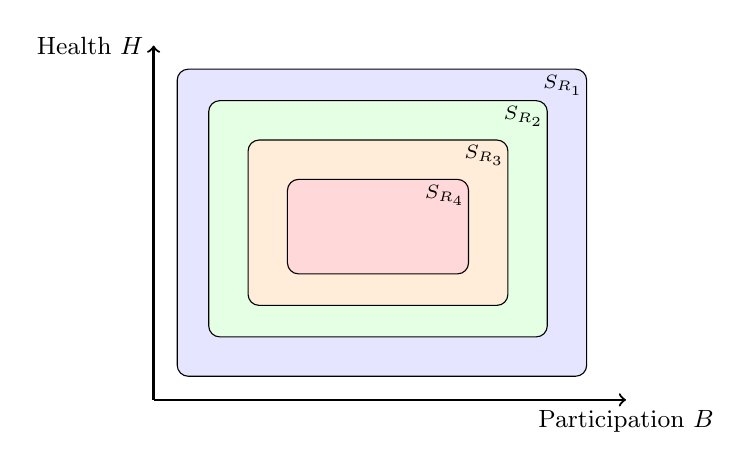
\begin{tikzpicture}[
    font=\small,
    axis/.style={->, thick},
    region/.style={draw, rounded corners},
]

% Axes
\draw[axis] (0,0) -- (0,4.5) node[left] {Health $H$};
\draw[axis] (0,0) -- (6,0) node[below] {Participation $B$};

% R1 (largest region)
\draw[region, fill=blue!10] (0.3,0.3) rectangle (5.5,4.2);
\node at (5.2,4) {\scriptsize $S_{R_1}$};

% R2
\draw[region, fill=green!10] (0.7,0.8) rectangle (5,3.8);
\node at (4.7,3.6) {\scriptsize $S_{R_2}$};

% R3
\draw[region, fill=orange!15] (1.2,1.2) rectangle (4.5,3.3);
\node at (4.2,3.1) {\scriptsize $S_{R_3}$};

% R4 (smallest)
\draw[region, fill=red!15] (1.7,1.6) rectangle (4,2.8);
\node at (3.7,2.6) {\scriptsize $S_{R_4}$};

\end{tikzpicture}

\caption{Reliability levels as progressively stricter admissible regions of the composite state space $S = B \times H$. Higher reliability levels permit fewer system configurations.}
\end{figure}